% Chapter Template

\chapter{Theoretical Background and Related Work} % Main chapter title

\label{Chapter2} % Change X to a consecutive number; for referencing this chapter elsewhere, use \ref{ChapterX}

The goal of this chapter is to provide the reader with the knowledge required to understand the rest of this work. As such I will not only talk about the theory behind the fingerprinting, ranging and triangulation methods but also describe the important characteristics of the observation parameters \red{and the smartphone(Android API)}. Where \red{helpful} I will also mention some of the related work or additional reading.
\note{rework this section: add comment for what I use the different technologies}

%----------------------------------------------------------------------------------------
%	SECTION 1
%----------------------------------------------------------------------------------------

\section{Observation parameters}

The observation parameters provide the information the rest of the approach is based on. Some of the important aspects to consider when choosing them are:
\begin{itemize}
\item They need to be available in an indoor environment.
\item They need to be detectable by the mobile device.
\item They need to contain some information suitable for localization.
\end{itemize}
Following the parameters are analyzed using these criteria.
\\\note{Rewrite this section/is is even necessary}
%-----------------------------------
%	SUBSECTION 1
%-----------------------------------
\subsection{RSSI and signal propagation}

The received signal strength indicator describes the total signal power received in milliwatts with the value expressed on a logarithmic scale (dBm)\cite[p.~160]{sauter2010gsm}. \red{In the case of Wi-Fi a value of -30 would mean a very strong signal while one of -90 would be so low as to be unusable (drowning in noise).}  In an open space without any obstacles the RSSI mainly depends on the propagation distance, but indoors several other factors become important. These are non line of sight (NLOS) and multipath propagation.

NLOS occurs when the signals path is obstructed by physical objects. The signal has to pass through these objects and therefore the RSSI is lower compared to LOS, where there are no obstacles\cite{JoseMaster}.

Multypath propagation is caused when the signal is reflected from physical objects and arrives at the receiver multiple times with different signal strength. This causes inaccuracy and fluctuations in the measured RSSI as all these signals are blended together\cite{multipathEffects}.

Both of these affects are very common in indoor environments, caused by the walls, people, furniture and other building materials. Furthermore the RSSI values are discrete and not fine grained what causes additional inaccuracy. This makes localization based on RSSI challenging and limits its accuracy.

There are other ways to assess the signal strength, such as channel state information, which is more fine grained and can mitigate multipath effects, but they are not available on most mobile devices\cite{JoseMaster,FineGrainedIndoorTracking}.

%-----------------------------------
%	SUBSECTION 2
%-----------------------------------

\subsection{Magnetic field in indoor environments}

Earths natural magnetic field has already been used for localization, mainly as a compass to determine the devices heading in PDR systems. However, the presence of magnetic field anomalies make accurate heading determination difficult for indoor applications. The anomalies are caused by the ferrous structures in the building materials, electrical devices, cables and tubes. Previous research suggests that these anomalies can be used in a fingerprinting approach to determine a devices location\cite{haverinen2009global,angermann2012CharacterizationMagnetic,Li2012feasableMagnetic}. They show that the magnetic field anomalies have sufficient local variability, are mostly stable over time and therefore applicable for use in localization.

In my case the magnetic field data is provided by the smartphones magnetometer sensor. It measures the magnetic field strength in microtesla along the devices three axis.\\
\note{Should I go more in depth here?}

\subsection{Smartphone hardware and \code{AndroidAPI}}

Smartphones are probably the most common mobile computing devices and they are usually equipped with many sensors; gyroscope, magnetometer, accelerometer, etc. This makes them a good target for indoor localization.But there are also some limitations when working with smartphones, especially concerning Wi-Fi.

In the case of Android, access to the devices Wi-Fi capability is limited by the \code{AndroidAPI}. \red{For} signal stength the RSSI is the only value provided, CSI is not supported. Also there is no way to only scan a single channel. A Wi-Fi scan has to be initiated through the \code{AndroidAPI} and it only supports full scans\cite{brouwers2014incremental}. Full scans take longer and so lower the sampling rate.

\red{Furthermore, because of the many different Wi-Fi modules and hardware configurations, the RSSI values measured by different Smartphones is not the same. This means that for every Smartphone type a new data set needs to be gathered.}

\note{Is this understandable?}

\red{Computing power can also be a limiting factor on older devices or when using more demanding algorithms.}

\note{rework this section}


%----------------------------------------------------------------------------------------
%	SECTION 2
%----------------------------------------------------------------------------------------

\section{Fingerprinting}

Fingerprinting is a common method for localization based on RSSI\cite{chapre2013RSSI}. It consists of two main phases.

In the offline/training phase a map of reference points (RP) is created by collecting RSSI values for each AN from known locations.
Then in the online phase RSSI values are collected from an unknown location, called the test point (TP). The location of the TP is determined based on the RP-map using machine learning algorithms like  a k-nearest neighbor regression\cite{JoseMaster}.

The accuracy of this method mainly depends on the density of the RP-map. The higher the density of RPs the better the accuracy. Generally achieving a satisfying level of accuracy, requires a lot of RPs. This is why this method is so labor intensive.

Other factors are the number of attributes in each RP and the variability of the observation parameters.

More attributes per RP, an attribute being a data value like a RSSI or a magnetic field measurement, gives the algorithm more information to work with and so increased the accuracy\cite{Li2012feasableMagnetic}. This effect is subject to diminishing returns\cite{brouwers2014incremental}.
\red{For the same reason a high variability in the observation parameters depending on location is also beneficial.}\note{citation needed}

\note{"For the same reason" is this understandable?}

\subsection{Support Vector Machine}
A Support Vector Machine (SVM) is a machine learning algorithm. It predicts the labels of new (unknown) samples based on previous (known) examples. \red{The set of labels is finite as it only supports two labels. This is called binary classification.}

The known examples are called training data. It consists of instance-label pairs \(\left ( x_{i}, y_{i} \right ), i=1,...,l\) where \(x_{i}\in R^{n}\) and \(y_{i}\in \left \{ -1,1 \right \}\). \(x_{i}\) represents the samples's observable features while the label \(y_{i}\) defines in which category it belongs.

The SVM maps the samples into \(n\)-dimentional space and then tries to fit a hyperplane through that space separating the two classes so that ideally all samples with \(y_{i}=1\) are on one side of the hyperplane and \(y_{i}=-1\) on the other. To make the separation as clear as possible the margin between the hyperplane and the samples is maximized at the same time. The samples which lie directly on the margins are called the support vectors.

To classify a new unknown sample the SVM determines on which side of the hyperplane it lies and assigns the according label.

\red{To fit the hyperpalane the SVM solves the following optimization} problem\cite{chang2011libsvm}:
\begin{equation}
\begin{split}
\min_{\omega , b ,\xi}\;\; & \frac{1}{2}\omega^{T}\omega +C\sum_{i=1}^{l}\xi_{i}\\
\textup{subject to}\;\; & y_{i}\left ( \omega^{T}\phi \left ( x_{i} \right )+b \right )\geq 1-\xi_{i},\\
& \xi_{i}\geq 0,i=1,...,l
\end{split}
\end{equation}

There may be outlines in the data, so a hyperplane that separates all samples correctly may not be the best classifier. To account for this, a cost is paid if a sample violates the error term \(y_{i}\left ( w^{T}\phi \left ( x_{i} \right )+b \right )\geq 1\), increasing the objective function by \(C \xi_{i}\). For large values of C the optimization will chose a hyperplane with a smaller margin, if it classifies more samples correctly. Conversely, a small value of C will cause the optimizer to look for a larger-margin separating hyperplane, even if that hyperplane misclassifies more samples\cite{crossValidatedSVMC}.

\begin{figure}[htp]

\label{fig:SVM}
\centering
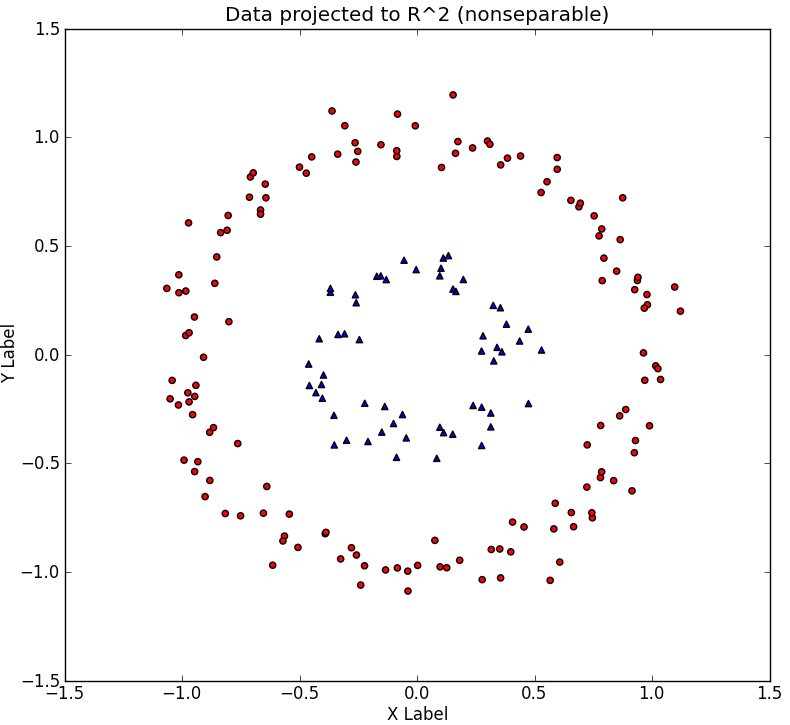
\includegraphics[width=.3\textwidth]{Figures/svm_1.png}\hfill
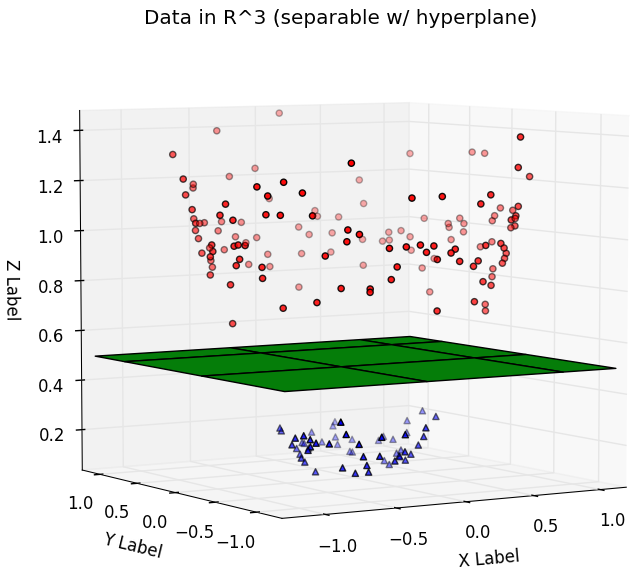
\includegraphics[width=.3\textwidth]{Figures/svm_2.png}\hfill
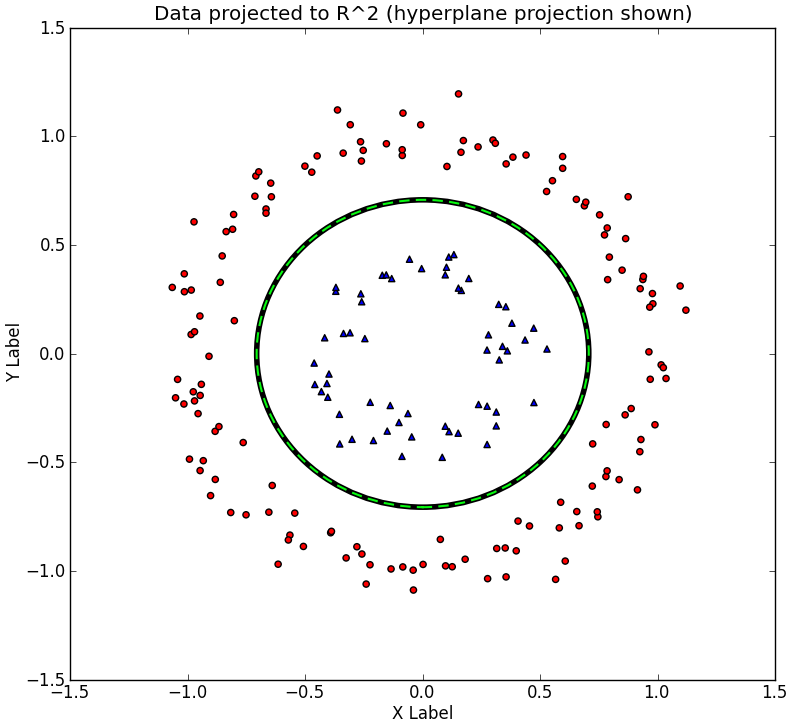
\includegraphics[width=.3\textwidth]{Figures/svm_3.png}
\decoRule
\caption[SVM kernel trick]{\raggedright(Left) A dataset in, not linearly separable. (Middle)The same dataset transformed with decision boundary. (Right) The nonlinear decision boundary.}

\end{figure}

But the training data may not be linearly separable. In this case the so called kernel trick can be used. The kernel is a function \(k\left ( x_{i}, x_{j} \right )=\phi \left ( x_{i} \right )\cdot \phi\left ( x_{j} \right )\) which maps the features \(x_{i}\) to a higher dimensional space where they can be separated by a hyperplane. This results in a non linear separation in the original feature space\cite{ErikKimKernelTrick}.

To perform multy-class classification the "one-against-one" approach can be used. For \(k\) classes \(k\left ( k-1 \right )/2\) classifiers are trained. Each binary classifier is then considered to vote for a class. The sample is then placed in the class with the most votes\cite{chang2011libsvm}.


\section{Ranging}
\label{Ranging}

The ranging process estimates the distance between the ANs and the MN based on the radio parameters, in this case RSSI. This is done with non-linear regression (NLR) and the following path loss model proposed by \cite{li2015passiveWIFIsource}:
\begin{equation} \label{eqn:non-linear path loss model}
d_{i}=\alpha_{i}e^{\beta_{i}RSSI_{i}}
\end{equation}
It describes the loss of signal strength over the propagation distance. \(d_{i}\) is the estimated distance from the MN to the \(i\)-th AN, \(RSSI_{i}\) is the \(i\)-th AN's signal strength as measured by the MN and \(\alpha_{i}, \beta_{i}\) are environment variables specific to each AN.

The model needs to be trained for each AN individually by determining the values for \(\alpha_{i}\) and \(\beta_{i}\). This is done by fitting the function to a small set of training samples \red{gathered from the building}. This can be done using any number of least squares optimization methods.

\section{Trilateration}

Trilateration is the process of determining a absolute or relative location based on the distance to known locations. In contrast to triangulation it relies on distances instead of angles.

In the context of localization the goal is to determine the NM's location \(\left ( x,y \right )\) based on the the locations of the ANs \(\left ( \tilde{x_{i}},\tilde{y_{i}} \right )\) and the distance estimations \(d_{i}\) obtained from the path loss model.

The actual distance \(D_{i}\) from the MN to the \(i\)-th AN can be expressed as follows:
\begin{equation}
D_{i} = \sqrt{\left ( \tilde{x_{i}}-x \right )^{2}+\left ( \tilde{y_{i}}-y \right )^{2}}
\label{eqn: distance MN to AN_{i}}
\end{equation}
Under the assumption that \(d_{i}=D_{i}\)  this leads to the following equation system:
\begin{equation}
\begin{pmatrix}
d_{1}\\ 
d_{2}\\
\vdots\\
d_{n}
\end{pmatrix}
=
\begin{pmatrix}
\sqrt{\left ( \tilde{x_{1}}-x \right )^{2}+\left ( \tilde{y_{1}}-y \right )^{2}}\\
\sqrt{\left ( \tilde{x_{2}}-x \right )^{2}+\left ( \tilde{y_{2}}-y \right )^{2}} \\
\vdots\\
\sqrt{\left ( \tilde{x_{n}}-x \right )^{2}+\left ( \tilde{y_{n}}-y \right )^{2}}
\end{pmatrix}
\label{eqn: trilateration problem as equation system}
\end{equation}

But \(d_{i}\) is only an estimation so there is no \red{exact} solution of the above system. The best solution is the one that minimizes the sum of the squared error \(d_{i} - D_{i}\). So to determine the MN's location the following problem has to be solved:
\begin{equation}
argmin_{x,y}\sum_{i=1}^{n}w_{i}\left ( d_{i} - \sqrt{\left ( \tilde{x_{i}}-x \right )^{2}+\left ( \tilde{y_{i}}-y \right )^{2}} \right )^{2}
\label{eqn: trilateration as optimization problem}
\end{equation}
This can be done using a optimization algorithm like "Levenberg–Marquardt" or "Gauss-Newton".

\red{The variance on the errors is not constant; Some distance estimation are more accurate than others. This can be taken into account with the set of weights \(w_{i}\) by applying a high weight to the more accurate estimations and a small weight to the inaccurate ones. This can improve the localization, but it is difficult determine the accuracy of the estimations.}
\note{should I add a separate subsection for Weighting?}
\note{These weights reflect how accurate the estimated distance to a AN is.}